\chapter{有限元求解器画廊}
\label{ch:gallery}

\begin{quote}
本章的目标是展示一系列重要的内容
科学与工程学院的PDEs可以很快得到解决
FEniCS代码行。 我们从热方程开始,继续
用非线性Poisson方程,线性方程
弹性,Navier-Stokes方程式,最后看看如何
解决非线性对流 - 扩散反应的系统
方程。 这些问题说明了如何解决时间依赖性问题
问题,非线性问题,向量值问题和系统
PDEs。 对于每个问题,我们得出变分公式
在Python中以非常类似的方式表达问题
数学。
\end{quote}

\section{热方程式}
\label{ch:fundamentals:diffusion}

\index{heat equation}
\index{time-dependent problem}

作为前一章的Poisson问题的第一个扩展,
我们考虑时间依赖热方程,或时间依赖性
扩散方程。 这是Poisson的自然延伸
描述体内热量的固定分布的方程式
时间依赖的问题。

我们会看到,通过将时间离散成小时间间隔
采用标准时间步法,可以解决热量
通过求解一系列变分问题的方程式,很像
一个我们遇到的Poisson方程。

\subsection{PDE问题}

我们的时间依赖型PDE的模型问题读取

\begin{alignat}{2}
{\partial u\over\partial t} &= \nabla^2 u + f \quad &&\hbox{in }\Omega\times(0, T],
\label{ch:diffusion0:pde1}\\
u &= \ub &&\hbox{on } \partial \Omega\times(0, T],
\label{ch:diffusion0:pde1:bc}\\
u &= \uI &&\mbox{at } t=0\tp
\label{ch:diffusion0:pde1:ic}
\end{alignat}
在这里,$u$随空间和时间而变化,例如,如果空间,则$u=u(x,y,t)$
域$\Omega$是二维的。 源函数$f$和
边界值$\ub$也可能因空间和时间而异。
初始条件$\uI$仅是空间的函数。

\subsection{变化公式}
\label{ftut:timedep:diffusion1}

一个简单的方法来解决时间依赖的PDEs
有限元方法是首先离散时间导数a
有限差分近似,产生一个序列
固定问题,然后将每个静止问题转化为
变分公式

让上标$n$表示时间$t_n$的数量,其中$n$是一个
整数计数时间级别。 例如,$u^n$表示$u$在时间
级$n$。 时间上的有限差分离散化包括
在某个时间级别对PDE进行采样,说$t_{n + 1}$:

\index{time step}

\begin{equation}
\left({\partial u \over\partial t}\right)^{n+1} = \nabla^2 u^{n+1} + f^{n+1}\tp
\label{ch:diffusion0:pde1:tk}
\end{equation}
时间导数可以通过差商近似。
为了简单和稳定的原因,我们选择一个
简单向后的差异:

\index{implicit Euler}
\index{backward difference}

\begin{equation}
\left({\partial u\over\partial t}\right)^{n+1}\approx {{u^{n+1} - u^n}\over{\dt}},
\label{ch:diffusion0:BE}
\end{equation}
其中$\dt$是时间离散参数。
(\ref{ch:diffusion0:pde1:tk})插入(\ref{ch:diffusion0:BE})产生

\begin{equation}
{{u^{n+1} - u^n}\over{\dt}} = \nabla^2 u^{n+1} + f^{n+1}\tp
\label{ch:diffusion0:pde1:BE}
\end{equation}
这是我们的时间离散版本的热方程
(\ref{ch:diffusion0:pde1}),所谓的\emph{backward Euler}或\emph{implicit
  Euler}离散化。

我们可以重新排序(\ref{ch:diffusion0:pde1:BE})
左侧包含未知$u^{n+1}$的条款
右侧仅包含计算的条件。 结果
是假设为$u^{n+1}$的空间(静态)问题的序列
$u^n$从以前的时间步长是已知的:

\begin{align}
u^0 &= \uI, \label{ch:diffusion0:pde1:u0}\\
u^{n+1} - {\dt}\nabla^2 u^{n+1} &=  u^n + {\dt} f^{n+1},\quad n=0,1,2,\ldots
\label{ch:diffusion0:pde1:uk}
\end{align}

给定$\uI$,我们可以解决$u^0$,$u^1$,$u^2$等。

(\ref{ch:diffusion0:pde1:uk})的替代方法,可以是
方便实施,是收集
平等标志一方的所有术语:

\begin{equation}
u^{n+1} - {\dt}\nabla^2 u^{n+1} -  u^{n} - {\dt} f^{n+1} = 0,\quad n=0,1,2,\ldots
\label{ch:diffusion0:pde1:uk2}
\end{equation}

我们使用有限元方法来解决
(\ref{ch:diffusion0:pde1:u0})和任一方程式
(\ref{ch:diffusion0:pde1:uk})或(\ref{ch:diffusion0:pde1:uk2})。 这个
需要将方程式变为弱形式。 像往常一样,我们倍增
通过一个测试函数$v\in \hat V$并将二阶导数合并
部分。 在$u^{n+1}$(这是自然的)中引入符号$u$
程序),由此产生的弱势形式
配方(\ref{ch:diffusion0:pde1:uk})
可以方便地写入
标准符号:

\[ a(u,v)=L_{n+1}(v),\]
哪里

\begin{align}
a(u,v) &= \int_\Omega\left(uv + {\dt}
\nabla u\cdot \nabla v\right) \dx, \label{ch:diffusion0:pde1:a}\\
L_{n+1}(v) &= \int_\Omega \left(u^n + {\dt}  f^{n+1}\right)v \dx\tp
\label{ch:diffusion0:pde1:L}
\end{align}
替代形式(\ref{ch:diffusion0:pde1:uk2})有一个
抽象配方

\[ F_{n+1}(u;v) = 0,\]
哪里

\begin{equation}
F_{n+1}(u; v) = \int_\Omega \left(uv + {\dt}
\nabla u\cdot \nabla v -
(u^n + {\dt} f^{n+1})v\right) \dx\tp
\label{ch:diffusion0:pde1:F}
\end{equation}

除了每个时间步长要解决的变化问题外,
我们还需要近似初始条件
(\ref{ch:diffusion0:pde1:u0})。 这个方程也可以变成a
变分问题:

\[ a_0(u,v)=L_0(v),\]
哪里

\begin{align}
a_0(u,v) &= \int_\Omega uv \dx, \label{ch:diffusion0:pde1:a0}\\
L_0(v) &= \int_\Omega \uI v \dx\tp \label{ch:diffusion0:pde1:L0}
\end{align}
当解决这个变分问题时,$u^0$成为$L^2$
将给定的初始值$\uI$投影到有限元中
空间。 另一种方式是通过内插来构造$u^0$
初始值$\uI$; 也就是说,如果$u^0=\sum_{j=1}^N U^0_j\phi_j$,我们
只需设置$U_j=\uI(x_j,y_j)$,其中$(x_j,y_j)$是坐标
节点编号$j$。 我们将这两个策略称为计算
初始条件通过投影或插值。 都
在FEniCS中通过单一语句轻松计算操作,
使用\texttt{project}或\texttt{interpolate}函数。 最常见的
选择是\texttt{project},它计算一个近似值为$\uI$,但是在
一些我们想通过再现来验证代码的应用程序
确切的解决方案,必须使用\texttt{interpolate}(我们使用这样的测试
这里的问题!)。

\index{interpolate@{\rm\texttt{interpolate}}}
\index{project@{\rm\texttt{project}}}

总之,我们需要解决以下变分序列
计算热方程有限元解的问题:
找到$u^0\in V$,以便$a_0(u^0,v)=L_0(v)$对于所有$v\in\hat V$,
然后找到$u^{n+1}\in V$
使得$a(u^{n+1},v)=L_{n+1}(v)$对于$v\in\hat V$,
或者,对于$v\in\hat V$中的$F_{n+1}(u^{n+1},v)=0$,
$n=0,1,2,\ldots$。

\subsection{FEniCS实现}
\label{ftut:timedep:diffusion1:impl}

我们的程序需要手动实现时间步伐,但可以
依靠FEniCS轻松计算$a_0$,$L_0$,$a$和$L$(或
$F_{n+1}$),并解决未知数的线性系统。

\paragraph{测试问题1:一个已知的分析解决方案。}
就像前一章的Poisson问题一样,我们
构建一个测试问题,使其容易确定是否
计算正确。 既然我们知道我们的一流
时间步长方案对于线性函数是精确的,我们创建一个测试
时间线性变化的问题。 我们把这与一个
空间二次变化。 我们因此而来

\begin{equation} u = 1 + x^2 + \alpha y^2 + \beta t,
\label{ch:diffusion0:pde1:u0test}
\end{equation}
其产生了在节点处的计算值将是的函数
确切的,不管元素的大小和$\dt$,只要
网格被均匀分割。 插入
(\ref{ch:diffusion0:pde1:u0test})转换为热方程
(\ref{ch:diffusion0:pde1}),我们发现右边的$f$必须
由$f(x,y,t)=\beta - 2 - 2\alpha$给出。 边界值
是$\ub(x,y,t)= 1 + x^2 + \alpha y^2 + \beta t$和初始
值为$\uI(x,y)= 1 + x^2 + \alpha y^2$。

\paragraph{FEniCS实现。}
一个新的编程问题是如何处理不同的功能
空间和时间,如边界条件$\ub(x,y,
t)= 1 + x^2 + \alpha y^2 + \beta t$。 一个自然的解决方案是使用
FEniCS \texttt{Expression}与time $t$作为参数,除了
参数$\alpha$和$\beta$:

\index{time-dependent expression}

\begin{python}
alpha = 3; beta = 1.2
u_D = Expression('1 + x[0]*x[0] + alpha*x[1]*x[1] + beta*t',
                 degree=2, alpha=alpha, beta=beta, t=0)
\end{python}
\texttt{Expression}将\texttt{x}的组件用作独立的
变量,而\texttt{alpha},\texttt{beta}和\texttt{t}是参数。该
time \texttt{t}可以稍后更新

\begin{python}
u_D.t = t
\end{python}

在这种情况下,沿着整个边界的基本边界条件,
以与我们以前实施的相同的方式实施
泊松问题的边界条件:

\begin{python}
def boundary(x, on_boundary):
    return on_boundary

bc = DirichletBC(V, u_D, boundary)
\end{python}

我们将使用变量\texttt{u}作为新的未知$u^{n+1}$
时间步长和变量\verb!u_n! 对于上一次的$u^n$
步。 \verb!u_n!的初始值可以通过任一投影来计算
或插值$\uI$。 由于我们为边界值设置了\texttt{t = 0}
\verb!u_D!,我们可以使用\verb!u_D! 指定初始条件:

\begin{python}
u_n = project(u_D, V)
# or
u_n = interpolate(u_D, V)
\end{python}

\begin{notice}[投影与内插初始条件]
实际恢复确切的解决方案
(\ref{ch:diffusion0:pde1:u0test})到机器精度,这很重要
通过内插$\uI$来计算离散的初始条件。 这个
确保自由度是准确的(机器精度)
在$t=0$。 投影导致节点处的近似值。
\end{notice}

\index{lhs@{\rm\texttt{lhs}}}
\index{rhs@{\rm\texttt{rhs}}}
\index{projection}
\index{interpolation}

我们可以根据上述公式定义$a$或$L$,或者我们
可能只是定义$F$,并要求FEniCS找出哪些术语应该去
进入双线性形式$a$,并且应该进入线性形式
$L$。 后者是方便的,特别是在更复杂的
问题,所以我们说明了建设$a$和$L$:

\begin{python}
u = TrialFunction(V)
v = TestFunction(V)
f = Constant(beta - 2 - 2*alpha)

F = u*v*dx + dt*dot(grad(u), grad(v))*dx - (u_n + dt*f)*v*dx
a, L = lhs(F), rhs(F)
\end{python}

最后,我们在循环中执行时间步长:

\begin{python}
u = Function(V)
t = 0
for n in range(num_steps):

    # Update current time
    t += dt
    u_D.t = t

    # Solve variational problem
    solve(a == L, u, bc)

    # Update previous solution
    u_n.assign(u)
\end{python}
在时间步长循环的最后一步,我们分配值
变量\texttt{u}(新计算的解决方案)变量\verb!u_n!
包含上一个时间步长的值。 必须这样做
使用\texttt{assign}成员函数。 如果我们反而尝试做\verb!u_n = u!,
我们将设置\verb!u_n! 变量与\texttt{u}变量相同
这不是我们想要的。 (我们需要两个变量,一个是值
在前一个时间步长,另一个是当前时间的值
步。)

\begin{notice}[记住用当前时间更新表达式对象!]
在时间循环内,观察\verb!u_D.t! 必须在之前更新
\texttt{solve}语句强制执行Dirichlet条件的计算
当前时间步长。 一个Dirichlet条件定义为a
\texttt{Expression}查找并应用参数的值,如\texttt{t}
当它被评估并应用于线性系统时。
\end{notice}

上面的时间步进循环不包含任何比较
数字和确切的解决方案,我们必须包括为了
验证实施。 至于Poisson方程式
部分~\ref{ch:poisson0:impl:dissect},我们计算差异
在\texttt{u}的节点数组和节点数组之间
内插精确解的值。 这可以做到
如下:

\begin{python}
u_e = interpolate(u_D, V)
error = np.abs(u_e.vector().array() - u.vector().array()).max()
print('t = %.2f: error = %.3g' % (t, error))
\end{python}
对于Poisson示例,我们使用了这个函数
\verb!compute_vertex_values! 提取功能值
顶点。 这里我们举例说明一种提取方法
顶点值,通过调用函数\texttt{vector}返回
自由度向量。 对于$\mathsf{P}_1$
功能空间,这个矢量的自由度将等于
通过调用获得的顶点值数组
\verb!compute_vertex_values!,虽然可能有不同的顺序。

解决热方程的完整程序如下:

\begin{python}
from fenics import *
import numpy as np

T = 2.0            # final time
num_steps = 10     # number of time steps
dt = T / num_steps # time step size
alpha = 3          # parameter alpha
beta = 1.2         # parameter beta

# Create mesh and define function space
nx = ny = 8
mesh = UnitSquareMesh(nx, ny)
V = FunctionSpace(mesh, 'P', 1)

# Define boundary condition
u_D = Expression('1 + x[0]*x[0] + alpha*x[1]*x[1] + beta*t',
                 degree=2, alpha=alpha, beta=beta, t=0)

def boundary(x, on_boundary):
    return on_boundary

bc = DirichletBC(V, u_D, boundary)

# Define initial value
u_n = interpolate(u_D, V)
#u_n = project(u_D, V)

# Define variational problem
u = TrialFunction(V)
v = TestFunction(V)
f = Constant(beta - 2 - 2*alpha)

F = u*v*dx + dt*dot(grad(u), grad(v))*dx - (u_n + dt*f)*v*dx
a, L = lhs(F), rhs(F)

# Time-stepping
u = Function(V)
t = 0
for n in range(num_steps):

    # Update current time
    t += dt
    u_D.t = t

    # Compute solution
    solve(a == L, u, bc)

    # Plot solution
    plot(u)

    # Compute error at vertices
    u_e = interpolate(u_D, V)
    error = np.abs(u_e.vector().array() - u.vector().array()).max()
    print('t = %.2f: error = %.3g' % (t, error))

    # Update previous solution
    u_n.assign(u)

# Hold plot
interactive()
\end{python}
该示例程序可以在文件中找到
\begin{center}
  \url{https://fenicsproject.org/pub/tutorial/python/vol1/ft03_heat.py}
\end{center}
\begin{center}
  {\nolinkurl{ft03_heat.py}}
\end{center}

\index{ft03\_heat.py@{\rm\texttt{ft03\_heat.py}}}

\paragraph{测试问题2:Gaussian函数的扩散。}
让我们现在解决一个更有趣的测试问题,即扩散
一个Gaussian山。 我们以初始值为准

\[ \uI(x,y)= e^{-ax^2 - ay^2}\]
在$a = 5$的域$[-2,2]\times [2,2]$。 为了这
问题我们将使用均匀的Dirichlet边界条件($\ub = 0$)。

\paragraph{FEniCS实现。}
以前的程序需要修改哪些? 一个专业
更改是域不再是单位平方。 新域名可以
使用\texttt{RectangleMesh}在FEniCS中轻松创建:

\begin{python}
nx = ny = 30
mesh = RectangleMesh(Point(-2, -2), Point(2, 2), nx, ny)
\end{python}
请注意,我们比以前使用了比以前更高的分辨率
解决解决方案的功能。 我们还需要重新定义
初始条件和边界条件。 两者都很容易改变
定义一个新的\texttt{Expression},并在边界上设置$u = 0$。

能够在外部程序中可视化解决方案,如
ParaView,我们将每次将解决方案保存为VTK格式的文件
步。 我们首先用后缀\texttt{.pvd}创建一个\texttt{File}:

\begin{python}
vtkfile = File('heat_gaussian/solution.pvd')
\end{python}
在时间循环中,我们可能会将解值附加到
这个文件:

\begin{python}
vtkfile << (u, t)
\end{python}
在每个时间步骤中调用此行,从而创建
一个包含后缀\texttt{.vtu}的新文件,其中包含时间步长的所有数据
(网格和顶点值)。 文件
\verb!heat_gaussian/solution.pvd! 将包含时间值和
引用\texttt{.vtu}文件,这意味着\texttt{.pvd}文件将是
单个小文件指向大量\texttt{.vtu}文件
包含实际数据。 请注意,我们选择存储解决方案
到一个名为\verb!heat_gaussian!的子目录。 这是为了避免混乱
我们的源目录与所有生成的数据文件。
在运行之前不需要创建目录
程序将由FEniCS自动创建。

\index{VTK format}
\index{.pvd@{\rm\texttt{.pvd}} file}
\index{.vtu@{\rm\texttt{.vtu}} file}

完整的程序如下所示。

\begin{python}
from fenics import *
import time

T = 2.0            # final time
num_steps = 50     # number of time steps
dt = T / num_steps # time step size

# Create mesh and define function space
nx = ny = 30
mesh = RectangleMesh(Point(-2, -2), Point(2, 2), nx, ny)
V = FunctionSpace(mesh, 'P', 1)

# Define boundary condition
def boundary(x, on_boundary):
    return on_boundary

bc = DirichletBC(V, Constant(0), boundary)

# Define initial value
u_0 = Expression('exp(-a*pow(x[0], 2) - a*pow(x[1], 2))',
                 degree=2, a=5)
u_n = interpolate(u_0, V)

# Define variational problem
u = TrialFunction(V)
v = TestFunction(V)
f = Constant(0)

F = u*v*dx + dt*dot(grad(u), grad(v))*dx - (u_n + dt*f)*v*dx
a, L = lhs(F), rhs(F)

# Create VTK file for saving solution
vtkfile = File('heat_gaussian/solution.pvd')

# Time-stepping
u = Function(V)
t = 0
for n in range(num_steps):

    # Update current time
    t += dt

    # Compute solution
    solve(a == L, u, bc)

    # Save to file and plot solution
    vtkfile << (u, t)
    plot(u)

    # Update previous solution
    u_n.assign(u)

# Hold plot
interactive()
\end{python}
该示例程序可以在文件中找到
\begin{center}
  \url{https://fenicsproject.org/pub/tutorial/python/vol1/ft04_heat_gaussian.py}
\end{center}
\begin{center}
  {\nolinkurl{ft04_heat_gaussian.py}}
\end{center}

\index{ft04\_heat\_gaussian.py@{\rm\texttt{ft04\_heat\_gaussian.py}}}

\paragraph{ParaView中的可视化。}
为了可视化高斯山的扩散,启动ParaView,
选择\textbf{File--Open...},打开
\verb!heat_gaussian/solution.pvd!,然后点击
\textbf{Apply}在Properties窗格中。 点击播放按钮进行显示
解决方案的动画。 要将动画保存到文件中,请单击
\textbf{File--Save Animation...}并将文件保存为所需的文件格式,
例如AVI或Ogg/Theora。
动画一旦保存到文件中,就可以播放动画
离线使用播放器,如mplayer或VLC,或上传您的
动画到YouTube。 图~\ref{fig:snapshots}显示了一个序列
的解决方案的快照。

%\begin{figure}[!ht]  % fig:snapshots
%  \centerline{
\includegraphics[width=0.95\linewidth]{fig/heat.png}}
%  \caption{
%  A sequence of snapshots of the solution of the Gaussian hill problem created with ParaView. \label{fig:snapshots}
%  }
%\end{figure}

\section{非线性Poisson方程}
\label{ftut1:gallery:nonlinearpoisson}

\index{nonlinear problem}

现在我们将介绍如何解决非线性PDE问题。 我们会看到
非线性问题可以像线性问题那样容易地解决
FEniCS,通过简单地定义非线性变分问题和调用
\texttt{solve}功能。 当这样做时,我们会遇到一个微妙的
变分问题如何定义的差异。

\subsection{PDE问题}

作为解决非线性PDE的模型问题,我们
取以下非线性Poisson方程:

\begin{equation}
-\nabla\cdot\left(q(u)\nabla u\right) = f,
\end{equation}
在$\Omega$中,$u=\ub$在边界$\partial\Omega$上。
系数$q = q(u)$使得方程非线性(除非$q(u)$
在$u$中是不变的)。

\subsection{变化公式}

像往常一样,我们的PDE乘以一个测试函数$v\in\hat V$,
整合域,并整合二阶导数
按部件。 由零件整合产生的边界积分
无论我们使用Dirichlet条件,都会消失。 所结果的
我们的模型问题的变分公式变成:找到$u \in V$
就这样

\begin{equation}
F(u; v) = 0 \quad \forall v \in \hat{V},
\label{ch:poisson0:nonlinear1}
\end{equation}
哪里

\begin{equation}
F(u; v) = \int_\Omega (q(u)\nabla u\cdot \nabla v - fv) \dx,
\label{ch:poisson0:nonlinear2}
\end{equation}
和

\begin{align*}
     V      &= \{v \in H^1(\Omega) : v = \ub \mbox{ on } \partial\Omega\},\\
    \hat{V} &= \{v \in H^1(\Omega) : v = 0 \mbox{ on } \partial\Omega\}\tp
\end{align*}

离散的问题像往常一样通过限制$V$和$\hat V$出现
到一对离散空间。 像以前一样,我们省略了任何下标
离散空间和离散解。
然后将离散的非线性问题写为:找到$u \in V$

\begin{equation}
  F(u; v) = 0 \quad \forall v \in \hat{V},
\label{ch:poisson0:nonlinear:d}
\end{equation}
与$u = \sum_{j=1}^N U_j \phi_j$。 由于$F$是非线性的
$u$,变量语句产生一个系统
未知数$U_1,\ldots,U_N$中的非线性代数方程。

\subsection{FEniCS实现}
\label{ftut:nonlinear:Newton:auto}

\paragraph{测试问题。}
为了解决测试问题,我们需要选择右边的$f$,
系数$q(u)$和边界值$\ub$。 以前,我们
与制造的解决方案一起工作,可以无需复制
近似误差 这在非线性问题上更为困难,
代数更加繁琐。 但是,我们可以利用SymPy
符号计算,并将这些计算集成到FEniCS中
求解。 这允许我们轻松地尝试不同的
制造解决方案。 SymPy的即将到来的代码需要一些
基本熟悉这个包。 特别是我们会用
SymPy函数\texttt{diff}用于符号区分和\texttt{ccode} for
C/C++代码生成。

我们取$q(u) = 1 + u^2$并定义二维制造
$x$和$y$中的线性解决方案:

\begin{python}
# Warning: from fenics import * will import both `sym` and
# `q` from FEniCS. We therefore import FEniCS first and then
# overwrite these objects.
from fenics import *

def q(u):
    "Return nonlinear coefficient"
    return 1 + u**2

# Use SymPy to compute f from the manufactured solution u
import sympy as sym
x, y = sym.symbols('x[0], x[1]')
u = 1 + x + 2*y
f = - sym.diff(q(u)*sym.diff(u, x), x) - sym.diff(q(u)*sym.diff(u, y), y)
f = sym.simplify(f)
u_code = sym.printing.ccode(u)
f_code = sym.printing.ccode(f)
print('u =', u_code)
print('f =', f_code)
\end{python}

\index{SymPy}
\index{method of manufactured solutions}

\begin{notice}[在\texttt{Expression}对象中根据需要定义符号坐标]
请注意,我们通常会写\texttt{x,y = sym.symbols('x,y')},但是
如果我们希望生成的表达式具有有效的语法
FEniCS \texttt{Expression}对象,我们必须使用\texttt{x[0]}和\texttt{x[1]}。
通过定义\texttt{x}的名称,\texttt{sympy}可以轻松实现这一点
\texttt{y} as \texttt{x[0]}和\texttt{x[1]}:\texttt{x,y = sym.symbols('x[0], x[1]')}。
\end{notice}

将\texttt{u}和\texttt{f}的表达式转换为C或C ++语法
FEniCS \texttt{Expression}对象需要两个步骤。 首先,我们要求C
表达式的代码:

\begin{python}
u_code = sym.printing.ccode(u)
f_code = sym.printing.ccode(f)
\end{python}
在某些情况下,需要编辑结果以匹配所需的结果
\texttt{Expression}对象的语法,但不是这种情况。 (首要的
例如\verb!M_PI! 对于$\pi$在C/C++中必须由\texttt{pi}替代
\texttt{Expression}对象。)在本例中,\verb!u_code!的输出 和
\verb!f_code!是

\begin{c}
x[0] + 2*x[1] + 1
-10*x[0] - 20*x[1] - 10
\end{c}
定义网格,功能空间和边界后,
我们定义边界值\verb!u_D! 如

\begin{python}
u_D = Expression(u_code, degree=1)
\end{python}
类似地,我们定义右边的函数

\begin{python}
f = Expression(f_code, degree=1)
\end{python}

\begin{notice}[命名FEniCS与程序变量之间的冲突]
在上面的程序中,可能会出现奇怪的错误
名字冲突。 如果在做之前定义\texttt{sym}和\texttt{q}
\texttt{from fenics import *},后一个语句也会导入
变量名为\texttt{sym}和\texttt{q},覆盖
你以前定义的对象! 这可能会导致奇怪
错误。 最安全的解决方案是做\texttt{import fenics}而不是
\texttt{from fenics import *},然后前缀所有FEniCS
\texttt{fenics}的对象名称。 下一个最好的解决办法就是做
\texttt{from fenics import *}首先定义你自己的变量
覆盖从\texttt{fenics}导入的那些。 这是可以接受的
如果我们不需要\texttt{fenics}中的\texttt{sym}和\texttt{q}。
\end{notice}

\paragraph{FEniCS实现。}
非线性Poisson方程的求解器很容易
实现线性Poisson方程的求解器。
我们所需要做的就是说明$F$和调用的公式
\texttt{solve(F == 0,u,bc)},而不是\texttt{solve(a == L,u,bc)}
在线性情况下。 这是一个简约代码:

\begin{python}
from fenics import *

def q(u):
    return 1 + u**2

mesh = UnitSquareMesh(8, 8)
V = FunctionSpace(mesh, 'P', 1)
u_D = Expression(u_code, degree=1)

def boundary(x, on_boundary):
    return on_boundary

bc = DirichletBC(V, u_D, boundary)

u = Function(V)
v = TestFunction(V)
f = Expression(f_code, degree=1)
F = q(u)*dot(grad(u), grad(v))*dx - f*v*dx

solve(F == 0, u, bc)
\end{python}

该示例程序的完整版本可以在该文件中找到
\begin{center}
\url{https://fenicsproject.org/pub/tutorial/python/vol1/ft05_poisson_nonlinear.py}
\end{center}
\begin{center}
{\nolinkurl{ft05_poisson_nonlinear.py}}
\end{center}

\index{ft05\_poisson\_nonlinear.py@{\rm\texttt{ft05\_poisson\_nonlinear.py}}}

与线性问题的主要区别在于未知功能
\texttt{u}在非线性情况下的变分形式
必须定义为\texttt{Function},而不是\texttt{TrialFunction}。 在某种意义上
这是从线性情况的简化,我们必须定义\texttt{u}
首先作为\texttt{TrialFunction}然后作为\texttt{Function}。

\index{Newton's method}
\index{Jacobian}

\texttt{solve}函数采用非线性方程,从符号出发
Jacobian矩阵,并运行一个Newton方法来计算解。

当我们运行代码时,FEniCS会报告Newton的进度
迭代。 以$2\cdot(8\times 8)$单元格,我们达到8的收敛
具有容忍度$10^{-9}$的迭代,以及错误
数值解约为$10^{-16}$。 这些结果带来了证据
为正确的实施。 思考有限差异
在均匀网格上,$\mathsf{P}_1$元素模拟标准
二阶差分,其计算线性的导数或
二次函数。 在这里,$\nabla u$是一个常量向量,但是
然后乘以$(1+u^2)$,它是二阶多项式
$x$和$y$,分歧“差异运算符”应该是
准确计算。 因此,我们可以使用$\mathcal{P}_1$
元素,期望制造的$u$被转载
数值方法。 像$1+u^4$这样的非线性,这不会是
情况,我们需要验证收敛率。

目前的例子显示了解决非线性问题的难易程度
在FEniCS。 但是,专家对非线性的数值解
PDEs非常了解,非线性的自动化程序可能会失败
问题,通常需要有更好的手册
解决方案的流程控制比我们目前的流程要好
案件。 我们在\cite{ftut2}中返回此问题,并显示如何
实现非线性方程式的定制解算法
我们如何引导使用的自动化Newton方法中的参数
以上。

\section{线性弹性方程}
\label{ftut:elast}

\index{elasticity}
\index{system of PDEs}

结构分析是现代主要活动之一
工程,这可能使PDE建模变形
弹性体是世界上最流行的PDE。 只需一个
用于解决FEniCS中2D或3D弹性方程的代码页,
具体细节如下。

\subsection{PDE问题}

\index{stress tensor}
\index{tensor}

控制身体的小弹性变形的方程式$\Omega$的方程式
可以写成

\begin{align}
-\nabla\cdot\sigma &= f\hbox{ in }\Omega,
\label{ftut:elast:varform:equilibrium}\\
\sigma &= \lambda\,\hbox{tr}\,(\varepsilon) I + 2\mu\varepsilon,
\label{ftut:elast:varform:stresstrain}\\
\varepsilon &= \frac{1}{2}\left(\nabla u + (\nabla u)^{\top}\right),
\label{ftut:elast:varform:strainu}
\end{align}
其中$\sigma$是压力张量,$f$是每单位的身体力量
卷,$\lambda$和$\mu$是$\text{Lam\'e's}$弹性参数为
物品在$\Omega$,$I$是身份张量,$\mathrm{tr}$是
跟踪运算符在张量上,$\varepsilon$是对称应变率
张量(对称梯度),$u$是位移矢量场。
我们这里假设各向同性弹性条件。

我们结合在一起 (\ref{ftut:elast:varform:stresstrain}) 和
(\ref{ftut:elast:varform:strainu}) 获得

\begin{equation}
\sigma = \lambda(\nabla\cdot u)I + \mu(\nabla u + (\nabla u)^{\top})\tp
\label{ftut:elast:varform:stressu}
\end{equation}
注意
(\ref{ftut:elast:varform:equilibrium})--(\ref{ftut:elast:varform:strainu})
可以轻松地转换为$u$的单个向量PDE,这是
管理未知$u$(Navier方程)的PDE。 在里面
然而,变分式的推导是方便的
保持方程式如上所述。

\subsection{变化公式}
\label{ftut:elast:varform}

变分公式
(\ref{ftut:elast:varform:equilibrium})--(\ref{ftut:elast:varform:strainu})
包括形成内部产品
(\ref{ftut:elast:varform:equilibrium})和一个\emph{vector}测试函数
$v\in \hat{V}$,其中$\hat{V}$是向量值的测试函数空间,
整合域$\Omega$:

\[ -\int_\Omega (\nabla\cdot\sigma) \cdot v \dx =
\int_\Omega f\cdot v\dx\tp\]
由于$\nabla\cdot\sigma $包含主要的二阶导数
未知$u$,我们将这个术语整合在一起:

\[ -\int_\Omega (\nabla\cdot\sigma) \cdot v \dx
= \int_\Omega \sigma : \nabla v\dx - \int_{\partial\Omega}
(\sigma\cdot n)\cdot v \ds,\]
冒号运算符是张量之间的内积(相加
所有元素的成对产品),$n$是向外单位正常
在边界。 数量$\sigma\cdot n$被称为
牵引力或应力矢量在边界,并经常规定
作为边界条件。 我们在这里假定它是在部分规定的
$\partial\Omega_T$的边界为$\sigma\cdot n = T$。 在上
剩下的一部分边界,我们假设的价值
位移作为Dirichlet条件给出。 我们得到了

\[
\int_\Omega \sigma : \nabla v \dx =
\int_\Omega f\cdot v \dx
+ \int_{\partial\Omega_T} T\cdot v\ds\tp\]
插入表达式(\ref{ftut:elast:varform:stressu})
$\sigma$给出$u$的变体形式为未知。 请注意
剩余部分的边界积分
由于Dirichlet,$\partial\Omega\setminus\partial\Omega_T$消失
条件。

我们现在可以将变分公式总结为:找到$u\in V$

\begin{equation}
a(u,v) = L(v)\quad\forall v\in\hat{V},
\end{equation}
哪里

\begin{align}
a(u,v) &= \int_\Omega\sigma(u) :\nabla v \dx,
\label{ftut:elast:varform:sigma_inner_gradv}
\\
\sigma(u) &= \lambda(\nabla\cdot u)I + \mu(\nabla u + (\nabla u)^{\top}),\\
L(v) &= \int_\Omega f\cdot v\dx + \int_{\partial\Omega_T}
T\cdot v\ds\tp
\end{align}

可以显示对称张量$A$和a的内积
反对称张量$B$消失。 如果我们表示$\nabla v$作为总和
的对称和反对称部分,只有对称部分
在产品$\sigma :\nabla v$中生存$\sigma$是a
对称张量。 因此用对称渐变替换$\nabla u$
$\epsilon(u)$产生略微不同的变化形式

\begin{equation}
a(u,v) = \int_\Omega\sigma(u) :\varepsilon(v) \dx,
\label{ftut:elast:varform:sigma_inner_eps}
\end{equation}
其中$\varepsilon(v)$是$\nabla v$的对称部分:

\[ \varepsilon(v) = \frac{1}{2}\left(\nabla v + (\nabla v)^{\top}\right)\tp\]
配方(\ref{ftut:elast:varform:sigma_inner_eps})是自然而然的
是由弹性势能的最小化引起的
流行的配方比(\ref{ftut:elast:varform:sigma_inner_gradv})。

\subsection{FEniCS实现}

\paragraph{测试问题。}
作为一个测试例子,我们将模拟在其下变形的夹紧梁
自重在3D。 这可以通过设置右侧来建模
每单位体积的身体力量$f=(0,0,-\varrho g)$ with $\varrho$ the
梁的密度和$g$重力加速度。 梁是
长度为$L$的盒形,宽度为$W$的正方形横截面。 我们
在夹紧的末端设置$u=\ub = (0,0,0)$,$x=0$。 其余的边界是
无牵引力 也就是说,我们设置$T = 0$。

\paragraph{FEniCS实现。}
我们首先列出代码,然后对新的结构进行评论
相比之前我们看到的例子。

\begin{python}
from fenics import *

# Scaled variables
L = 1; W = 0.2
mu = 1
rho = 1
delta = W/L
gamma = 0.4*delta**2
beta = 1.25
lambda_ = beta
g = gamma

# Create mesh and define function space
mesh = BoxMesh(Point(0, 0, 0), Point(L, W, W), 10, 3, 3)
V = VectorFunctionSpace(mesh, 'P', 1)

# Define boundary condition
tol = 1E-14

def clamped_boundary(x, on_boundary):
    return on_boundary and x[0] < tol

bc = DirichletBC(V, Constant((0, 0, 0)), clamped_boundary)

# Define strain and stress

def epsilon(u):
    return 0.5*(nabla_grad(u) + nabla_grad(u).T)
    #return sym(nabla_grad(u))

def sigma(u):
    return lambda_*nabla_div(u)*Identity(d) + 2*mu*epsilon(u)

# Define variational problem
u = TrialFunction(V)
d = u.geometric_dimension()  # space dimension
v = TestFunction(V)
f = Constant((0, 0, -rho*g))
T = Constant((0, 0, 0))
a = inner(sigma(u), epsilon(v))*dx
L = dot(f, v)*dx + dot(T, v)*ds

# Compute solution
u = Function(V)
solve(a == L, u, bc)

# Plot solution
plot(u, title='Displacement', mode='displacement')

# Plot stress
s = sigma(u) - (1./3)*tr(sigma(u))*Identity(d)  # deviatoric stress
von_Mises = sqrt(3./2*inner(s, s))
V = FunctionSpace(mesh, 'P', 1)
von_Mises = project(von_Mises, V)
plot(von_Mises, title='Stress intensity')

# Compute magnitude of displacement
u_magnitude = sqrt(dot(u, u))
u_magnitude = project(u_magnitude, V)
plot(u_magnitude, 'Displacement magnitude')
print('min/max u:',
      u_magnitude.vector().array().min(),
      u_magnitude.vector().array().max())
\end{python}
该示例程序可以在文件中找到
\begin{center}
  \url{https://fenicsproject.org/pub/tutorial/python/vol1/ft06_elasticity.py}
\end{center}
\begin{center}
  {\nolinkurl{ft06_elasticity.py}}
\end{center}

\index{ft06\_elasticity.py@{\rm\texttt{ft06\_elasticity.py}}}

\paragraph{向量函数空间。}
\index{vector-valued functions}
\index{VectorFunctionSpace@{\rm\texttt{VectorFunctionSpace}}}

主要的未知数现在是矢量字段$u$而不是标量字段,
所以我们需要使用向量函数空间:

\begin{python}
V = VectorFunctionSpace(mesh, 'P', 1)
\end{python}
使用\texttt{u = Function(V)},我们得到\texttt{u}作为向量值有限元
功能与这个3D问题的三个组件。

\paragraph{恒定向量。}
对于边界条件$u=(0,0,0)$,我们必须设置一个向量值
为零,不仅仅是一个标量。 这样的向量常数被指定为
\texttt{Constant((0,0,0))}在FEniCS中。 相应的2D代码将使用
\texttt{Constant((0,0))}。 在代码中,我们还需要\texttt{f}作为向量
并指定为\texttt{Constant((0,0,rho*g))}。

%\paragraph{\protect\verb!nabla\_grad!.}
\index{nabla\_grad@{\rm\texttt{nabla\_grad}}}

渐变和差异运算符现在有一个前缀\verb!nabla_!
这在目前的问题上是绝对不必要的,但是
一般推荐由连续力学引起的载体PDE,
如果您将$\nabla$解释为PDE表示法中的向量;
看到关于\verb!nabla_grad!的框 在~\ref{ftut1:NS:varform}中。

\paragraph{压力计算。}
一旦计算了位移\texttt{u},我们可以计算各种
压力措施。 我们将计算von Mises应力定义为
$\sigma_M = \sqrt{\frac{3}{2}s:s}$其中$s$是偏差应力
张量

\[ s = \sigma - \frac{1}{3}\mathrm{tr}\,(\sigma)\,I\tp\]
这些公式和FEniCS代码之间存在一对一的映射:

\begin{python}
s = sigma(u) - (1./3)*tr(sigma(u))*Identity(d)
von_Mises = sqrt(3./2*inner(s, s))
\end{python}
\verb!von_Mises! 变量现在是必须预计的表达式
有限元空间,我们可以看到它:

\begin{python}
V = FunctionSpace(mesh, 'P', 1)
von_Mises = project(von_Mises, V)
plot(von_Mises, title='Stress intensity')
\end{python}

\paragraph{缩放。}
\index{scaling}

经常
有利于缩小问题,因为它减少了设置的需要
物理参数,一个获得无量纲的数字
反映参数和物理效应的竞争。 我们开发
具有尺寸的原始模型的代码,并运行缩放
通过适当调整参数的问题。 缩放减少
本应用程序的活动参数数目为6到2。

在Navier的$u$方程中,由插入产生
(\ref{ftut:elast:varform:stresstrain})和
(\ref{ftut:elast:varform:strainu})成
(\ref{ftut:elast:varform:equilibrium}),

\[ -(\lambda + \mu)\nabla(\nabla\cdot u) - \mu\nabla^2 u = f,\]
我们插入由$L$制成的维度坐标,$\bar u=u/U$,
这导致无量纲控制方程

\[
-\beta\bar\nabla(\bar\nabla\cdot \bar u) - \bar\nabla^2 \bar u =
\bar f,\quad \bar f = (0,0,\gamma),\]
其中$\beta = 1 + \lambda/\mu$是无量纲弹性参数
哪里

\[ \gamma = \frac{\varrho gL^2}{\mu U}\]
是反映负载比率的无量纲变量
$\varrho g$和剪切应力
在PDE中的期限$\mu\nabla^2u\sim \mu U/L^2$。

缩放的一个选项是选择$U$,使$\gamma$为
单位大小($U = \varrho gL^2/\mu$)。然而,在弹性方面,这导致
到几何尺寸的位移,这使得地块
看起来很奇怪因此,我们想要特征位移
是几何特征长度的一小部分。
这可以通过选择$U$等于最大偏转来实现
实际上存在一个公式:$U =
\frac{3}{2}\varrho gL^2\delta^2/E$,其中$\delta = L/W$是
参数反映梁的细长度,$E$是模数
的弹性。因此,无量纲参数$\delta$非常
在问题上重要(如预期的那样,因为$\delta\gg 1$是什么
  给出光束理论!)。以$E$为$\mu$相同的顺序,
这是许多材料的情况,我们意识到$\gamma \sim
\delta^{-2}$是一个合适的选择。试验代码
在变形的地块中找到“看起来正确”的位移
几何,指向$\gamma = 0.4\delta^{-2}$作为我们的最终选择
$\gamma$。

模拟代码实现了维度的问题
物理参数$\lambda$,$\mu$,$\varrho$,$g$,$L$和$W$。
但是,我们可以轻松地重用这个代码来解决一个缩放的问题:只需设置
$\mu = \varrho = L = 1$,$W$ 如 $W/L$ ($\delta^{-1}$),$g=\gamma$和
$\lambda=\beta$。

%\begin{figure}[!ht]  %
%  \centerline{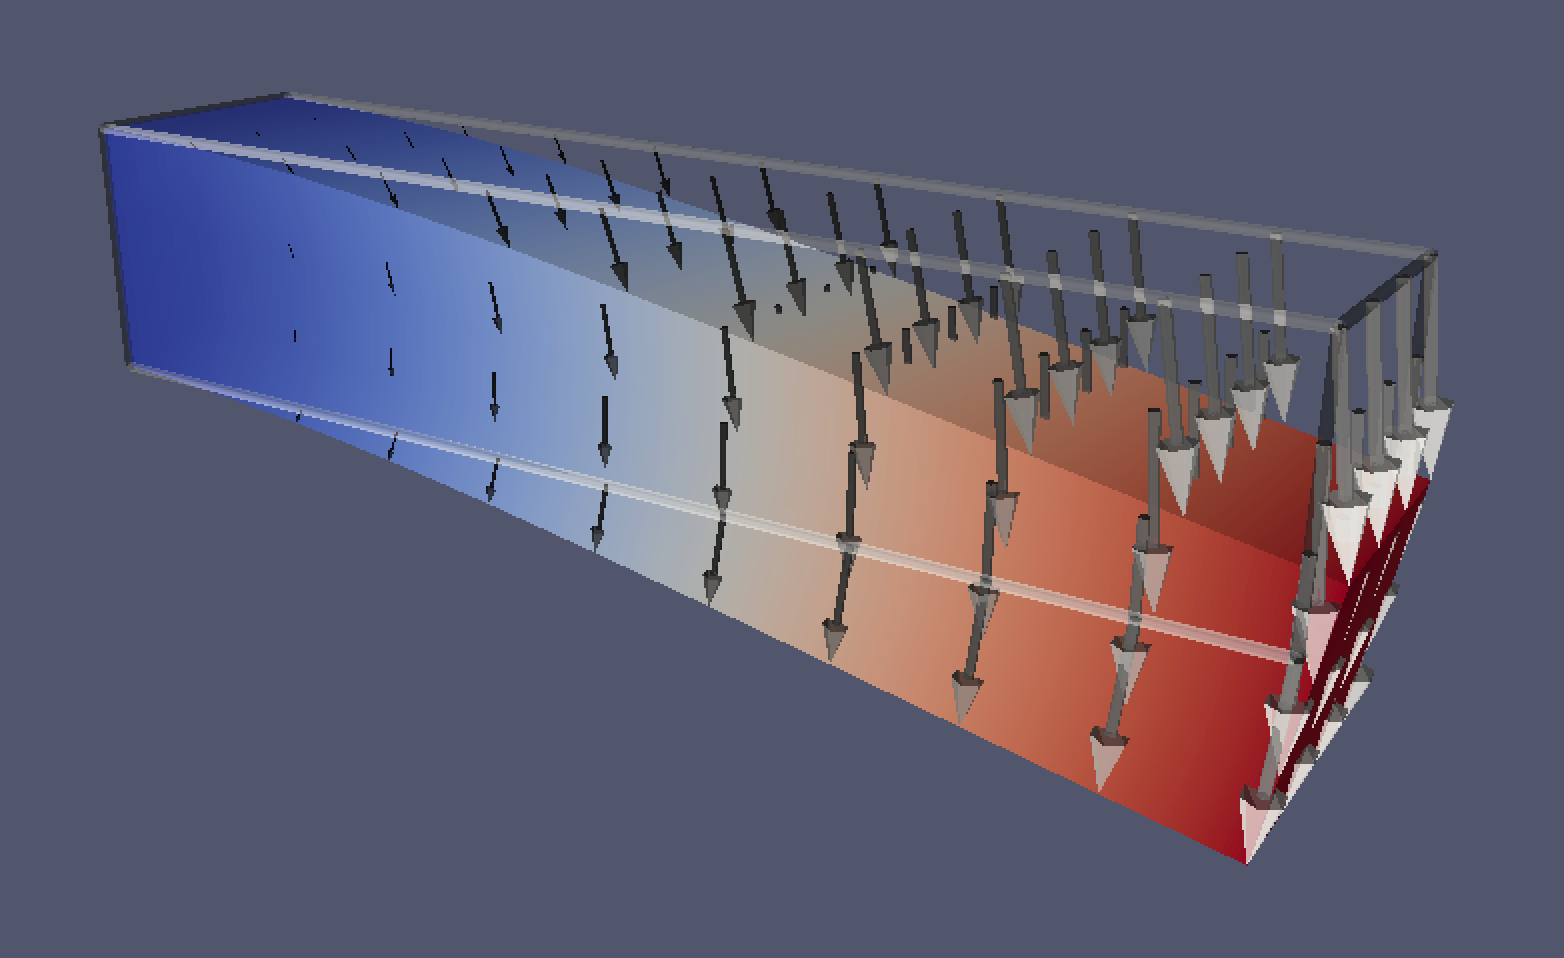
\includegraphics[width=0.95\linewidth]{fig/elasticity.png}}
%  \caption{
%  Plot of gravity-induced deflection in a clamped beam for the elasticity problem.
%  }
%\end{figure}

\section{Navier--Stokes方程}
\label{ftut1:NS}

\index{Navier-Stokes equations}
\index{CFD}

对于下一个例子,我们将解决不可压缩的Navier--Stokes
方程。 这个问题结合了我们的许多挑战
以前研究过的问题:时间依赖,非线性和
向量值变量。 我们将介绍一些FEniCS主题,
其中许多相当先进。 但你会看到,即使是相对的
复杂算法如二阶分割方法
不可压缩的Navier--Stokes方程,可以实现
FEniCS相对容易。

\subsection{PDE问题}

不可压缩的Navier--Stokes方程组成一个方程组
对于不可压缩流体的速度$u$和压力$p$:

\begin{align}
  \label{ftut1:ns:momentum}
  \varrho\left(\frac{\partial u}{\partial t} +
  u \cdot \nabla u\right) &= \nabla\cdot\sigma(u, p) + f, \\
  \label{ftut1:ns:continuity}
  \nabla \cdot u &= 0.
\end{align}
右边的$f$是每单位体积的给定力量
就线性弹性方程而言,
$\sigma(u,p)$表示应力张量,对于Newtonian流体
是(谁)给的

\index{stress tensor}

\begin{equation}
  \sigma(u, p) = 2\mu\epsilon(u) - pI,
\end{equation}
其中$\epsilon(u)$是应变率张量

\index{strain-rate tensor}

\[ \epsilon(u) = \frac{1}{2}\left(\nabla u + (\nabla u)^T\right)\tp\]
参数$\mu$是动态粘度。 注意势头
方程(\ref{ftut1:ns:momentum})非常类似于弹性
方程(\ref{ftut:elast:varform:equilibrium})。 区别在于
两个附加条款$\varrho(\partial u/ \partial t + u \cdot \ nabla u)$和不同的
表达式为应力张量。 两个额外的术语表达
加速平衡的力量$F = \nabla\cdot\sigma + f$每单位体积在Newton第二运动定律。
